\documentclass[12pt]{article}

\usepackage{sbc-template}
\usepackage{graphicx,url}
\usepackage[utf8]{inputenc}
\usepackage[T1]{fontenc}
\usepackage[brazil]{babel}

\sloppy

\graphicspath{{figuras/}}

\title{Métricas DORA em repositórios open-source populares do GitHub}

\author{Brenda Evers\inst{1}, Carlos José Gomes Batista Figueiredo\inst{1}, Gabriela Alvarenga Cardoso\inst{1}}

\address{Pontifícia Universidade Católica de Minas Gerais (PUC Minas)\\
Belo Horizonte -- MG -- Brasil
\email{\{1523565, 1507022, 1026227\}@pucminas.edu.br}
}

\begin{document}

\maketitle

\begin{abstract}
  The DORA metrics are the standard for measuring software delivery performance, but public repositories do not record deployments or production failures, so they must be inferred from proxies. We mined deployment frequency, lead time, change failure rate and recovery time from 300 popular GitHub repositories that use GitHub Actions, over one year, and validated our corrective-release heuristic against a manually labeled gold standard of 60 repositories (F1 of 0.644). Repositories deploy a median of 0.54 releases per week, with a median lead time of about 11 days, a CI-based failure rate of 4.7\% and a recovery time of 2.6 hours. Repository age is the factor most associated with performance. Changing the operational definition moves 22\% to 30\% of repositories to a different DORA category (weighted kappa of 0.54 to 0.69), so repository-level classifications should be read as estimates.
\end{abstract}

\begin{resumo}
  As métricas DORA são o padrão para medir o desempenho de entrega de software, mas repositórios públicos não registram deploys nem falhas em produção, e é preciso inferi-los por aproximações. Mineramos a frequência de deploy, o lead time, a taxa de falha de mudanças e o tempo de recuperação de 300 repositórios populares do GitHub que usam GitHub Actions, em um ano, e validamos a heurística de release corretiva contra uma amostra-ouro rotulada manualmente, com 60 repositórios (F1 de 0,644). Os repositórios publicam uma mediana de 0,54 releases por semana, com lead time mediano de cerca de 11 dias, taxa de falha de CI de 4,7\% e recuperação em 2,6 horas. A idade do repositório é o fator mais associado ao desempenho. Mudar a definição operacional leva de 22\% a 30\% dos repositórios a outra categoria DORA (kappa ponderado de 0,54 a 0,69), de modo que a classificação de cada repositório deve ser lida como estimativa.
\end{resumo}

\section{Introdução}

As métricas DORA (\textit{DevOps Research and Assessment})~--- frequência de deploy, lead time, taxa de falha de mudanças (CFR, \textit{Change Failure Rate}) e tempo de recuperação~--- tornaram-se a referência para medir o desempenho de entrega de software \cite{forsgren2018accelerate}. Elas classificam equipes em quatro faixas (\textit{Elite}, \textit{High}, \textit{Medium} e \textit{Low}) e associam entrega rápida e estável a melhores resultados organizacionais \cite{dora2024report}. Apesar disso, a maior parte da evidência vem de pesquisas com questionários respondidos por profissionais, e pouco se sabe sobre como projetos open-source populares se posicionam nessas faixas quando as métricas são calculadas a partir dos próprios dados do repositório.

O problema é que, em repositórios públicos, as métricas DORA não são observadas diretamente: o GitHub não registra deploys nem falhas em produção, e é preciso inferi-los a partir de aproximações (\textit{proxies}), como releases, commits e execuções de \textit{workflows} do GitHub Actions. Cada escolha de definição (o que conta como deploy, como identificar uma falha, quando há recuperação) pode alterar a classificação de um repositório, e não há consenso sobre qual operacionalização é a mais adequada.

O objetivo deste trabalho é mensurar as quatro métricas DORA em repositórios populares do GitHub que usam GitHub Actions, em uma janela de um ano (01/10/2025 a 30/09/2026), e investigar como elas se relacionam entre si, como variam com características dos repositórios e quão sensíveis são às definições adotadas. Para isso, formulamos oito questões de pesquisa (RQ 01 a RQ 08): as RQ 01 a RQ 04 descrevem cada métrica; a RQ 05 trata da relação entre frequência de deploy e taxa de falha; a RQ 06, das características dos repositórios associadas a melhor desempenho; a RQ 07, da sensibilidade da classificação às definições; e a RQ 08 (bônus), do \textit{rework rate}. As hipóteses de cada questão, escritas antes da coleta e da análise dos dados, são apresentadas a seguir.

\paragraph{RQ 01 (frequência de deploy).}
Esperamos que a faixa \textit{Medium} (de uma release por mês a uma por semana) seja a mais comum, que a \textit{High} reúna uma parcela menor e que só uma minoria alcance a \textit{Elite} (sete ou mais por semana). Muitos projetos open-source fazem releases manuais ou por marcos, e estrelas indicam visibilidade, não cadência de entrega, de modo que a distribuição deve ser assimétrica. Como o critério de inclusão exige cinco releases na janela, a faixa \textit{Low} deve reunir os repositórios com cinco a onze releases no ano.

\paragraph{RQ 02 (lead time).}
Esperamos lead times medianos de dias a poucas semanas, com a maioria dos repositórios nas faixas \textit{Medium} e \textit{High}, porque as releases acumulam commits por semanas. A variante (a), medida a partir do commit mais antigo da release, deve dar valores maiores e mais repositórios na faixa \textit{Low} que a (b), já que basta um commit antigo ``esquecido'' para elevá-la; na (b), cada commit entra com o próprio lead time. Em ambas, a distribuição deve ter cauda longa.

\paragraph{RQ 03 (taxa de falha de mudanças, CFR).}
Esperamos CFR baixo para a maior parte dos repositórios, nas faixas \textit{Elite} (até 15\%) ou \textit{High} (até 30\%), com grande dispersão. A variante (a), de execuções de CI com falha, deve ser maior que a (b), de releases corretivas, porque inclui testes instáveis e problemas de infraestrutura que nunca chegam ao usuário.

\paragraph{RQ 04 (tempo de recuperação).}
Esperamos que a maior parte das falhas seja recuperada em menos de um dia, já que corrigir o CI costuma exigir um commit pequeno, com mediana na faixa \textit{High} e poucos repositórios \textit{Elite}. Esperamos também IQR amplo, cauda de episódios de dias ou semanas em projetos pouco ativos e uma parcela de episódios censurados.


\paragraph{RQ 05 (frequência de deploy e taxa de falha).}
Para o CFR (a), esperamos correlação de Spearman fraca ($|\rho| < 0{,}3$) com a frequência de deploy, em linha com o DORA, para quem velocidade e estabilidade não são um \textit{trade-off} \cite{dora2024report}: a proporção de execuções com falha depende mais dos testes e da infraestrutura do CI que da cadência de releases. Para o CFR (b), esperamos correlação positiva e moderada, em parte por construção: quem publica várias releases por semana quase sempre tem outra em até 7 dias, e basta que ela seja corretiva para a anterior contar como falha. As duas variantes devem, portanto, levar a conclusões diferentes.

\paragraph{RQ 06 (características associadas ao desempenho).}
Esperamos as associações mais fortes com o número de contribuidores, que traz mais mudanças e mais pessoas para corrigir falhas, e com o tipo do projeto, já que bibliotecas publicam \textit{patches} frequentes no GitHub e aplicações costumam entregar por outros canais. Para popularidade, linguagem e idade, esperamos diferenças pequenas: todos os repositórios já são populares, e estrelas medem visibilidade, não processo. Esperamos efeitos pequenos a médios e poucas comparações significativas após a correção de Holm.

\paragraph{RQ 07 (sensibilidade às definições).}
Esperamos que a classificação geral mude para 20\% a 40\% dos repositórios em cada par de combinações, quase sempre para uma categoria vizinha, com kappa ponderado moderado a substancial. C2 e C3 devem levar a categorias melhores que C1, porque pré-releases e tags aumentam a frequência de deploy e o lead time (b) tende a ser menor que o (a). A maior divergência deve ser em C1$\times$C2 e a menor em C2$\times$C3. Como a categoria geral é a mediana de quatro notas, a variação por métrica deve ser maior que a da classificação geral.

\paragraph{RQ 08 (\textit{rework rate} e evolução temporal).}
Esperamos \textit{rework rate} mediano entre 20\% e 40\%, maior que o CFR (b) e fortemente correlacionado com ele: o CFR (b) só atribui a falha à release corrigida em até 7 dias, enquanto o \textit{rework rate} conta as próprias releases corretivas, inclusive as posteriores a esse prazo. Na evolução temporal, esperamos que quase nenhum repositório tenha tendência significativa: com quatro trimestres, o teste de Mann-Kendall bilateral não atinge $p < 0{,}05$ (o menor p-valor possível é cerca de 0,09).



\section{Metodologia}

\subsection{Fonte de dados e seleção}

Os dados vêm da API do GitHub (REST e, para as tags, GraphQL), consultada por um \textit{pipeline} em Python com cache em disco, que espera a renovação da cota e pode ser reexecutado sem novas requisições. A busca por repositórios com mais de 1.000 estrelas é dividida em faixas de estrelas, para contornar o teto de 1.000 resultados por consulta. Os candidatos são percorridos por estrelas decrescente até o 300º aprovado. Um repositório entra se usa o GitHub Actions, se publicou ao menos 5 releases na janela e se teve ao menos 50 execuções de \textit{workflow} válidas (com sucesso ou falha) no \textit{default branch}. A janela vai de 01/10/2025 a 30/09/2026, em UTC. Dos 5.620 candidatos encontrados, 712 foram examinados: 70 não usam o Actions, 296 têm menos de 5 releases e 46 têm menos de 50 execuções, restando 300. Como a seleção segue a ordem de estrelas, a amostra reúne os repositórios mais populares que passam no funil, e não é um sorteio (de 40.681 a 391.478 estrelas, mediana de 62.559). Como a API devolve no máximo 1.000 execuções por consulta, a janela é consultada mês a mês, e os meses que atingem o teto são refeitos por dia e por hora.

\subsection{Definições operacionais}
\label{sec:definicoes}

Um \textit{deploy} é uma release publicada na janela que não é rascunho nem pré-release. As métricas, calculadas por repositório, são:

\begin{itemize}
\item \textbf{Frequência de deploy:} deploys divididos pelas 52,14 semanas da janela.
\item \textbf{Lead time:} tempo entre um commit e a publicação da release que o inclui. Na variante (a), cada release conta uma vez, com o seu commit mais antigo; na (b), conta cada commit. O resultado é a mediana do repositório.
\item \textbf{CFR:} na variante (a), a proporção de execuções com falha entre as com sucesso ou falha, o que mede falha de CI e não de produção. Na (b), a proporção de releases seguidas, em até 7 dias, por uma release corretiva (Seção~\ref{sec:validacao}); as releases cujos 7 dias seguintes não cabem na janela ficam fora.
\item \textbf{Tempo de recuperação:} em cada \textit{workflow}, o tempo entre a primeira falha e o sucesso seguinte, com a mediana dos episódios completos. Episódios que não terminam na janela, ou que já começam falhando, são censurados e não entram na mediana, mas são contados.
\item \textbf{\textit{Rework rate}:} proporção de releases corretivas entre as avaliadas.
\end{itemize}

Cada métrica recebe uma nota de 4 (\textit{Elite}) a 1 (\textit{Low}) por cortes adaptados do relatório DORA \cite{dora2024report} (por exemplo, \textit{Elite} é 7 ou mais deploys por semana, lead time abaixo de 1 dia, CFR de até 15\% e recuperação abaixo de 1 hora). A categoria geral é a mediana das notas das métricas definidas, arredondada para baixo. A combinação C1 usa a frequência por release, o lead time (a) e o CFR (a); a C2 conta também as pré-releases como deploys e usa o lead time (b) e o CFR (b); e a C3 conta tags no lugar de releases e usa o lead time (b) e o CFR (a). A recuperação é a mesma nas três.

\subsection{Validação manual}
\label{sec:validacao}

A heurística de release corretiva e o tipo de projeto foram validados contra uma amostra-ouro de 60 repositórios, sorteados com semente fixa (42) da lista de aprovados previstos, com 5 releases sorteadas de cada um (300 releases). Os três autores rotularam a amostra de forma independente, sem ver a saída da heurística, segundo um protocolo escrito antes do sorteio: o tipo do projeto, se as releases são entregas reais ao usuário e se cada release é corretiva, a partir das \textit{release notes} e dos commits. O consenso é o rótulo da maioria, que existiu em todos os itens; os 55 itens com divergência (2--1) foram revisados em reunião, e nenhum rótulo mudou.

O kappa de Fleiss, calculado antes do consenso, foi de 0,82 no tipo do projeto (quase perfeita), 0,19 nas entregas reais (leve) e 0,78 nas releases corretivas (substancial), segundo Landis e Koch \cite{landis1977measurement}. O valor baixo em entregas reais decorre da prevalência do rótulo ``sim'' (54 a 59 dos 60 repositórios): os três avaliadores concordaram em 53 deles (88\%). A heurística foi avaliada contra o consenso das 300 releases (73 corretivas). A versão 1, baseada no número da versão e em palavras-chave nos commits, teve F1 de 0,415; a versão 2, que lê as \textit{release notes}, 0,606; e a versão 3, que lê as notas por seção e exige maioria de commits de correção, 0,644 (precisão de 0,632 e \textit{recall} de 0,658). A meta de 0,70 não foi atingida, e a versão 3 é a usada nos resultados.

\subsection{Análise estatística}

As métricas são resumidas por mediana e intervalo interquartil. A RQ 05 usa a correlação de Spearman entre a frequência de deploy e cada variante do CFR. Na RQ 06, cada métrica é comparada entre os grupos de cada fator (linguagem, tipo do projeto, e quartis de estrelas, de contribuidores e de idade) pelo teste de Kruskal-Wallis ou, com dois grupos, de Mann-Whitney, com correção de Holm sobre todos os testes (nível de 0,05) e tamanho de efeito $\varepsilon^2$ ou $\delta$ de Cliff. O tipo do projeto só existe para os 60 repositórios da amostra-ouro, e grupos com menos de 5 valores ficam fora. A RQ 07 compara as categorias de cada par de combinações pelo percentual que muda e pelo kappa de Cohen ponderado linear.


\section{Resultados das RQ 01 a RQ 04}

Os resultados descrevem os 300 repositórios da amostra. As métricas, muito assimétricas, são resumidas por mediana e IQR (Tabela~\ref{tab:descritiva}) e classificadas nas faixas DORA (Figura~\ref{fig:faixas}), e a Tabela~\ref{tab:hipoteses} resume o veredito de cada hipótese. Na classificação geral (C1), 24 repositórios (8,0\%) são \textit{Elite}, 131 (43,7\%) \textit{High}, 130 (43,3\%) \textit{Medium} e 15 (5,0\%) \textit{Low}; em 17, uma das quatro métricas não pôde ser calculada, e a categoria usa as demais.

\begin{table}[ht]
\centering
\small
\caption{Estatísticas descritivas das métricas (n = repositórios com valor definido; Indef. = repositórios sem valor).}
\label{tab:descritiva}
\begin{tabular}{lrrrrrrr}
\hline
Métrica & n & Indef. & Mediana & Q1 & Q3 & Mín. & Máx. \\
\hline
Deploys por semana & 300 & 0 & 0,54 & 0,25 & 1,23 & 0,10 & 49,56 \\
Lead time (a), h & 299 & 1 & 255,7 & 73,2 & 952,8 & 0,01 & 50\,634 \\
Lead time (b), h & 299 & 1 & 277,0 & 77,2 & 1\,250,7 & 0,01 & 107\,152 \\
CFR (a), \% & 300 & 0 & 4,7 & 2,3 & 11,1 & 0,0 & 90,1 \\
CFR (b), \% & 298 & 2 & 17,4 & 5,9 & 32,8 & 0,0 & 88,1 \\
Recuperação, h & 284 & 16 & 2,56 & 0,98 & 6,59 & 0,07 & 181,8 \\
Episódios censurados, \% & 289 & 11 & 1,1 & 0,0 & 5,3 & 0,0 & 100,0 \\
\hline
\end{tabular}
\end{table}

\begin{figure}[ht]
\centering
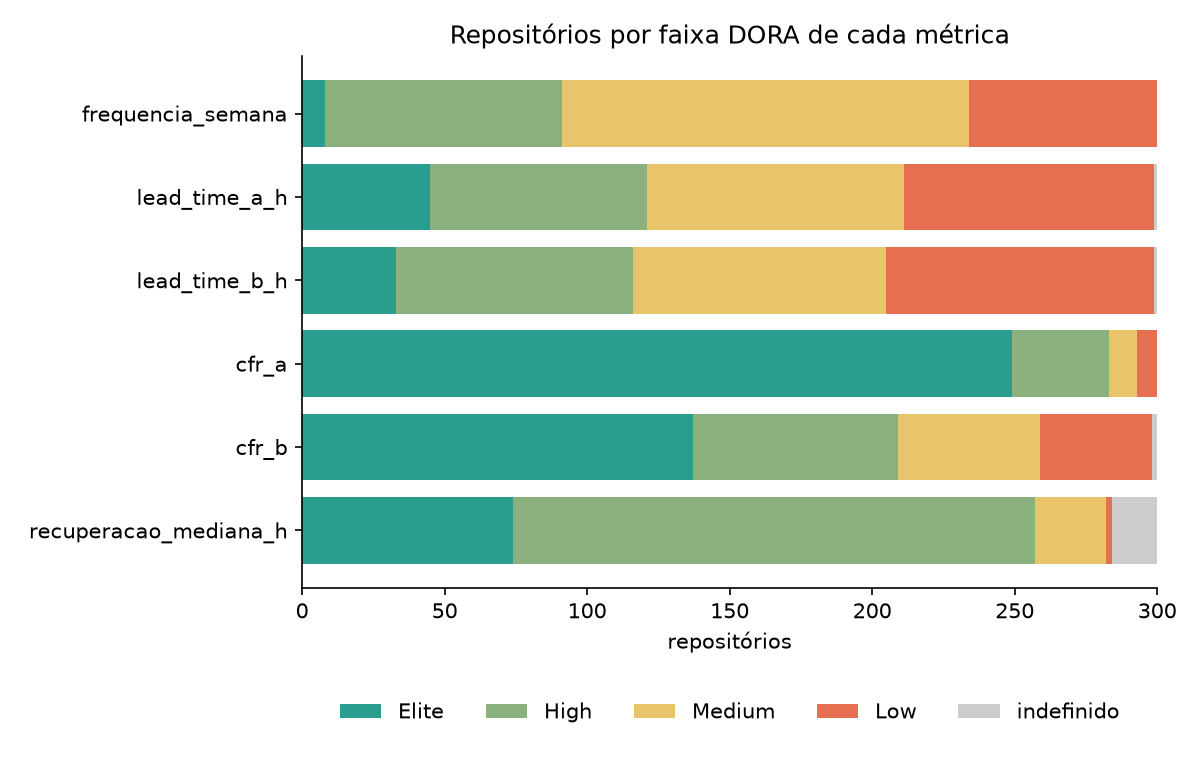
\includegraphics[width=0.75\textwidth]{faixas_por_metrica.png}
\caption{Repositórios por faixa DORA em cada métrica (cinza: métrica indefinida).}
\label{fig:faixas}
\end{figure}

\begin{table}[t]
\centering
\small
\caption{Hipóteses das RQ 01 a RQ 04 frente aos resultados.}
\label{tab:hipoteses}
\begin{tabular}{p{0.04\textwidth}p{0.50\textwidth}p{0.38\textwidth}}
\hline
RQ & Hipótese & Resultado \\
\hline
01 & \textit{Medium} mais comum, \textit{Elite} minoria, \textit{Low} com 5 a 11 releases & Confirmada (\textit{Medium} com 45\%) \\
02 & Dias a poucas semanas, na maioria \textit{Medium} e \textit{High} & Confirmada \\
02 & Variante (a) maior e com mais \textit{Low} que a (b) & Refutada (88 \textit{Low} contra 94) \\
03 & CFR baixo na maioria, com grande dispersão & Confirmada \\
03 & CFR (a) maior que CFR (b) & Refutada (4,7\% contra 17,4\%) \\
04 & Menos de um dia, mediana \textit{High}, com censura & Confirmada \\
04 & Poucos \textit{Elite}, IQR amplo e cauda de dias a semanas & Parcial (26,1\% \textit{Elite}; IQR estreito) \\
\hline
\end{tabular}
\end{table}

\subsection{RQ 01: frequência de deploy}

A faixa \textit{Medium} reúne 135 repositórios (45,0\%), seguida da \textit{High} (83; 27,7\%), da \textit{Low} (74; 24,7\%) e da \textit{Elite} (8; 2,7\%), e o repositório mais frequente publica 49,6 releases por semana, quase cem vezes a mediana. A \textit{Medium} é maioria relativa, e não absoluta. Chama a atenção a cauda lenta: um quarto dos projetos populares publica menos de uma release por mês, o que reforça que estrelas não indicam cadência de entrega.

\subsection{RQ 02: lead time}

O lead time mediano é de 10,7 dias na variante (a) e de 11,5 dias na (b), com distribuições parecidas: na (a), 45 repositórios são \textit{Elite}, 76 \textit{High}, 90 \textit{Medium} e 88 \textit{Low}; na (b), 33, 83, 89 e 94. A variante (a) é maior em 58,9\% dos repositórios, mas por pouco, e a diferença não aparece na distribuição agregada. Uma explicação plausível, não testada, é que a (b) pondera cada commit e dá mais peso às releases grandes, enquanto a (a) dá o mesmo peso a cada release.

\subsection{RQ 03: taxa de falha de mudanças}

No CFR (a), 83,0\% dos repositórios são \textit{Elite}; no CFR (b), 46,0\% são \textit{Elite}, 24,2\% \textit{High}, 16,8\% \textit{Medium} e 13,1\% \textit{Low}. Ao contrário do esperado, a variante (a) é menor em 67,1\% dos repositórios, provavelmente porque divide as falhas por todas as execuções de CI, enquanto a (b) divide por poucas releases (mediana de 28). A (a) mede falha de \textit{pipeline}, e não de produção; a (b) se aproxima mais do DORA, mas depende da heurística de release corretiva (Seção~\ref{sec:validacao}) e deve ser lida como estimativa ruidosa.

\subsection{RQ 04: tempo de recuperação}

Dos 284 repositórios com valor, 90,5\% se recuperam em menos de um dia: 26,1\% são \textit{Elite}, 64,4\% \textit{High}, 8,8\% \textit{Medium} e 0,7\% \textit{Low}. Dezesseis ficam sem valor, por não terem episódio de falha completo, e 0,9\% dos 64\,672 episódios são censurados. A cauda longa esperada não aparece (só 2 repositórios chegam a uma semana, e o IQR é estreito), e os \textit{Elite} são mais de um quarto.


\section{Resultados das RQ 05 e RQ 06}

\subsection{RQ 05: frequência de deploy e taxa de falha}

A correlação de Spearman entre a frequência de deploy e o CFR (a) é positiva e fraca ($\rho = 0{,}162$; $p = 0{,}005$; $n = 300$), e com o CFR (b) é positiva e forte pela magnitude de Cohen ($\rho = 0{,}501$; $p < 0{,}001$; $n = 298$), no limite com a faixa moderada. A Figura~\ref{fig:rq05} mostra os dois gráficos. Há muitos empates em zero: 11 repositórios têm CFR (a) igual a 0 e 61 têm CFR (b) igual a 0, que recebem o posto médio.

\begin{figure}[ht]
\centering
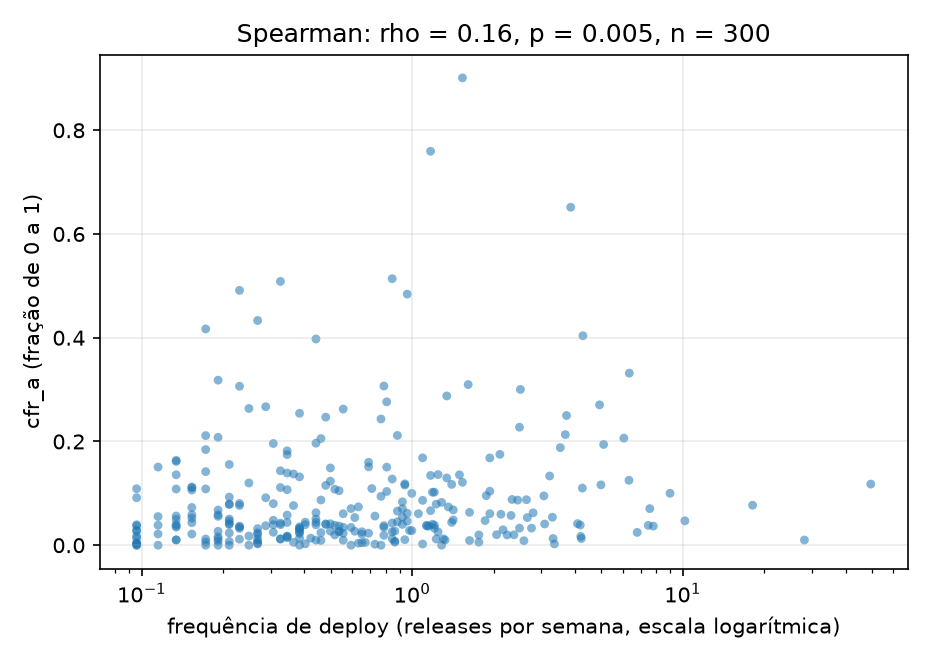
\includegraphics[width=0.48\textwidth]{rq05_cfr_a.png}\hfill
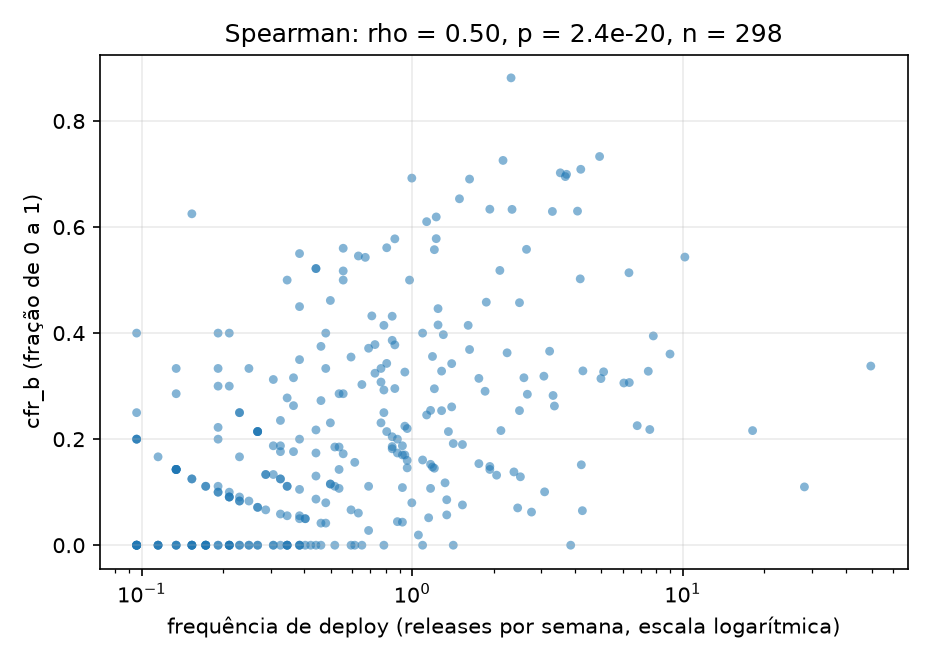
\includegraphics[width=0.48\textwidth]{rq05_cfr_b.png}
\caption{Frequência de deploy (escala logarítmica) e CFR de cada repositório: variante (a), à esquerda, e variante (b), à direita.}
\label{fig:rq05}
\end{figure}

Confirmamos as duas hipóteses. Para o CFR (a), a correlação é fraca ($|\rho| < 0{,}3$), de modo que a frequência de deploy explica pouco da taxa de falha de CI (cerca de 3\% da variação dos postos). O sinal é positivo e significativo, e não nulo: quem publica mais releases tem um pouco mais de execuções com falha. Para o CFR (b), a correlação positiva e moderada que esperávamos ficou no limite entre moderada e forte. As duas variantes levam a conclusões diferentes sobre o \textit{trade-off} entre velocidade e estabilidade: o CFR (a) indica quase independência, em linha com o DORA \cite{dora2024report}, e o CFR (b) indica que mais releases vêm com mais correções. Esse segundo resultado é em parte efeito da definição, pois quem publica mais releases tem mais chance de ter uma correção em até 7 dias, e não deve ser lido como prova de que a velocidade causa instabilidade.

\subsection{RQ 06: características associadas ao desempenho}

Foram feitos 20 testes (cinco fatores e quatro métricas), e só 4 continuam significativos após a correção de Holm, todos com $p < 0{,}001$ (Tabela~\ref{tab:rq06}). A idade tem o maior efeito: os repositórios mais novos publicam mais releases e têm lead time menor. Com mais contribuidores, o lead time também é maior. A linguagem se associa ao lead time com efeito médio. Nenhum fator se associa significativamente ao CFR (a) nem ao tempo de recuperação, e a popularidade (estrelas) e o tipo do projeto não mostram associação significativa com nenhuma métrica ($p$ ajustado de 0,54 a 1,0; o tipo cobre só 58 repositórios, 54 na recuperação).

\begin{table}[ht]
\centering
\small
\caption{Comparações significativas após a correção de Holm (todas com $p < 0{,}001$) e medianas por grupo. Os quartis de idade vão de 110 a 931 dias (Q1) até 3.936 a 6.746 dias (Q4), e os de contribuidores, de 8 a 223 (Q1) até 1.070 a 9.908 (Q4).}
\label{tab:rq06}
\begin{tabular}{llrp{0.32\textwidth}}
\hline
Fator e métrica & $\varepsilon^2$ & n & Mediana por grupo \\
\hline
Idade e lead time (a) & 0,365 (grande) & 299 & Q1 a Q4: 51, 204, 477 e 1.024 h \\
Contribuidores e lead time (a) & 0,183 (médio) & 299 & Q1 a Q4: 131, 179, 220 e 981 h \\
Idade e frequência & 0,118 (médio) & 300 & Q1 a Q4: 0,94, 0,61, 0,35 e 0,36 por semana \\
Linguagem e lead time (a) & 0,095 (médio) & 299 & Python 131 h, TypeScript 217 h e Rust 183 h; Go 567 h e outras 658 h \\
\hline
\end{tabular}
\end{table}

Confirmamos que poucas comparações permanecem significativas (4 de 20), e que a popularidade e o tamanho do efeito da maioria são pequenos. As demais expectativas não se confirmaram. Esperávamos as maiores associações com os contribuidores e o tipo do projeto, mas a maior foi com a idade, que prevíamos pequena, e o tipo do projeto não apresentou nenhuma. Os contribuidores se associam ao lead time, mas no sentido oposto ao esperado: os projetos com mais contribuidores levam mais tempo, e não menos, para publicar o que foi escrito, sem efeito na frequência nem na recuperação. Uma explicação plausível, que não testamos, é que projetos mais antigos e maiores têm processos de release mais cautelosos e mais commits acumulados entre uma release e outra. A análise por fator isolado não separa idade e contribuidores, que podem andar juntos, e o tamanho do efeito da idade (grande) sugere que ela é o fator mais importante da amostra.


\section{Resultados da RQ 07}

A RQ 07 compara a classificação geral dos repositórios nas combinações C1, C2 e C3 (Seção~\ref{sec:definicoes}), repositório a repositório, pelo percentual que muda de categoria e pelo kappa de Cohen ponderado linear. Ficam fora do par os repositórios com C2 ou C3 indefinida: \texttt{zed-industries/zed} (sem lead time (b) e CFR (b) em C2) e \texttt{docling-project/docling} (sem as tags de C3), porque a API devolveu HTTP 422 em uma consulta de cada um. Por isso os pares têm 299, 299 e 298 repositórios.

\begin{table}[ht]
\centering
\small
\caption{Concordância entre as classificações gerais de cada par de combinações (Mudam = repositórios que trocam de categoria; Vizinha = trocas de uma só categoria; Sobem e Descem = sentido da troca de $x$ para $y$).}
\label{tab:rq07_pares}
\begin{tabular}{lrrrrrrl}
\hline
Par ($x \times y$) & n & Mudam & \% & Vizinha & Sobem & Descem & $\kappa$ \\
\hline
C1 $\times$ C2 & 299 & 90 & 30,1 & 83 & 26 & 64 & 0,544 (moderada) \\
C1 $\times$ C3 & 299 & 65 & 21,7 & 61 & 49 & 16 & 0,685 (substancial) \\
C2 $\times$ C3 & 298 & 85 & 28,5 & 82 & 81 & 4 & 0,591 (moderada) \\
\hline
\end{tabular}
\end{table}

Entre 21,7\% e 30,1\% dos repositórios mudam de categoria conforme a definição (Tabela~\ref{tab:rq07_pares}), 92\% a 97\% delas para uma categoria vizinha, e nenhum vai de \textit{Elite} para \textit{Low}, ou o contrário. A Figura~\ref{fig:rq07} mostra que, em C1$\times$C2, só 6 dos 24 repositórios \textit{Elite} de C1 continuam \textit{Elite} (13 passam a \textit{High} e 5 a \textit{Medium}), enquanto em C1$\times$C3 17 dos 24 continuam.

\begin{figure}[ht]
\centering
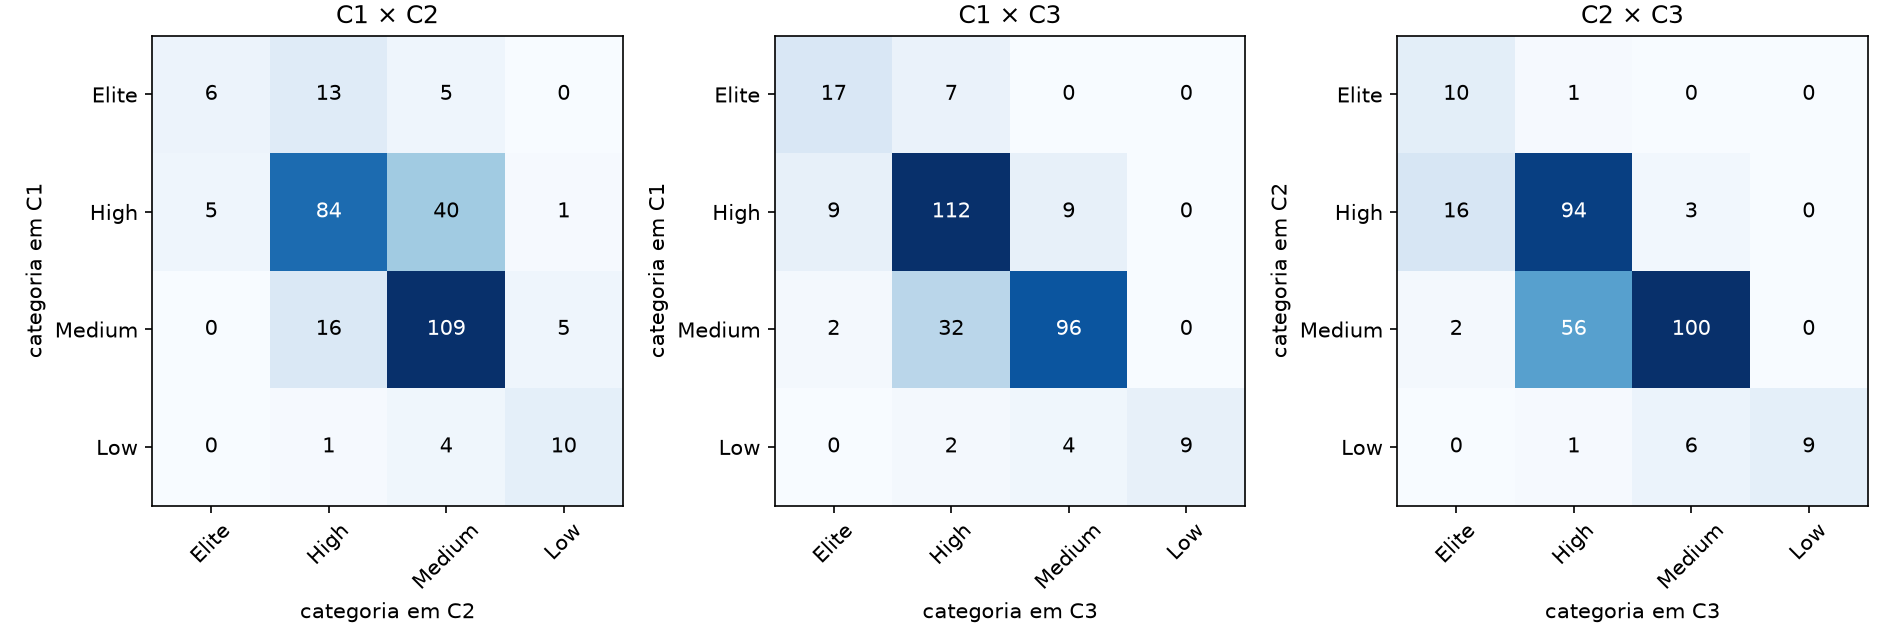
\includegraphics[width=0.88\textwidth]{rq07_matrizes.png}
\caption{Matrizes de transição entre as categorias gerais de cada par de combinações (as linhas são a categoria na primeira combinação, e as colunas, na segunda).}
\label{fig:rq07}
\end{figure}

A distribuição agregada também muda: os \textit{Elite} são 24 em C1, 11 em C2 e 28 em C3, e a categoria mais comum é a \textit{High} em C1 (por um repositório) e em C3 (51,2\%), mas a \textit{Medium} em C2 (52,8\%).

\begin{table}[ht]
\centering
\small
\caption{Mudança de faixa de cada métrica entre as combinações: \% de repositórios cuja nota muda e, entre parênteses, quantos sobem e quantos descem de $x$ para $y$. O CFR de C1 e C3 é o mesmo (CFR (a)).}
\label{tab:rq07_metricas}
\begin{tabular}{lrrr}
\hline
 & C1 $\times$ C2 & C1 $\times$ C3 & C2 $\times$ C3 \\
\hline
Frequência de deploy & 10,7 (32/0) & 25,1 (75/0) & 15,1 (45/0) \\
Lead time & 43,6 (66/64) & 46,6 (75/64) & 10,1 (21/9) \\
CFR & 59,3 (29/147) & 0,0 (0/0) & 59,3 (147/29) \\
Classificação geral & 30,1 (26/64) & 21,7 (49/16) & 28,5 (81/4) \\
\hline
\end{tabular}
\end{table}

A Tabela~\ref{tab:rq07_metricas} mostra de onde vêm as trocas. O CFR muda de faixa em 59,3\% dos repositórios entre C2 e as demais, quase sempre para pior em C2, cujo CFR (b) tem mediana de 17,0\%, contra 4,7\% do (a). O lead time muda em 43,6\% a 46,6\% entre C1 e as demais, nos dois sentidos (medianas de 255,7 h em C1, 264,1 h em C2 e 215,6 h em C3), mas em só 10,1\% entre C2 e C3, que usam a mesma variante. A frequência só sobe: a mediana passa de 0,54 para 0,65 (C2) e 0,88 (C3) por semana. Como a categoria geral é a mediana de quatro notas, parte das trocas é absorvida.

\begin{table}[t]
\centering
\small
\caption{Hipóteses da RQ 07 frente aos resultados.}
\label{tab:hipoteses_rq07}
\begin{tabular}{p{0.55\textwidth}p{0.37\textwidth}}
\hline
Hipótese & Resultado \\
\hline
20\% a 40\% mudam de categoria em cada par & Confirmada (21,7\% a 30,1\%) \\
Mudanças quase sempre para uma categoria vizinha & Confirmada (92\% a 97\%) \\
Kappa ponderado moderado a substancial & Confirmada (0,544 a 0,685) \\
C2 e C3 levam a categorias melhores que C1 & Confirmada só para C3 \\
Pré-releases e tags aumentam a frequência & Confirmada \\
Lead time (b) menor que o (a) & Parcial: só em C3 \\
Maior divergência em C1$\times$C2, menor em C2$\times$C3 & Parcial: a menor é C1$\times$C3 \\
Variação por métrica maior que a da geral & Parcial: não na frequência \\
\hline
\end{tabular}
\end{table}

\subsection{Discussão}

A escolha da definição não inverte o desempenho de um repositório, mas desloca a categoria de cerca de um em quatro e muda a categoria mais comum. Só C3 leva a categorias melhores, porque em C2 a piora do CFR supera o ganho de frequência; e a menor divergência é em C1$\times$C3, porque o que importa não é quantas definições os pares compartilham, mas quais: C1 e C3 compartilham o CFR (a), a métrica que mais muda de faixa. Para as RQ 01 a RQ 06, os valores por repositório devem ser lidos como estimativas, mas as conclusões gerais se mantêm: os repositórios seguem concentrados em \textit{High} e \textit{Medium} nas três combinações.


\section{Resultados da RQ 08}

Escolhemos a opção do \textit{rework rate} e não analisamos a evolução temporal, que a hipótese da RQ 08 também previa. O \textit{rework rate} tem mediana de 31,1\% (IQR de 14,2\% a 52,5\%), e 29 repositórios o têm igual a zero. O CFR (b) tem mediana de 17,4\% (IQR de 5,9\% a 32,8\%). O \textit{rework rate} é maior que o CFR (b) em 223 dos 298 repositórios com as duas métricas, menor em 19 e igual em 56 (diferença significativa pelo teste de Wilcoxon pareado unilateral, $p < 0{,}001$, e correlação \textit{rank-biserial} de 0,97). A correlação de Spearman entre os dois é positiva e forte ($\rho = 0{,}706$; $n = 298$). A Figura~\ref{fig:rq08} mostra que a maioria dos repositórios fica acima da diagonal.

\begin{figure}[ht]
\centering
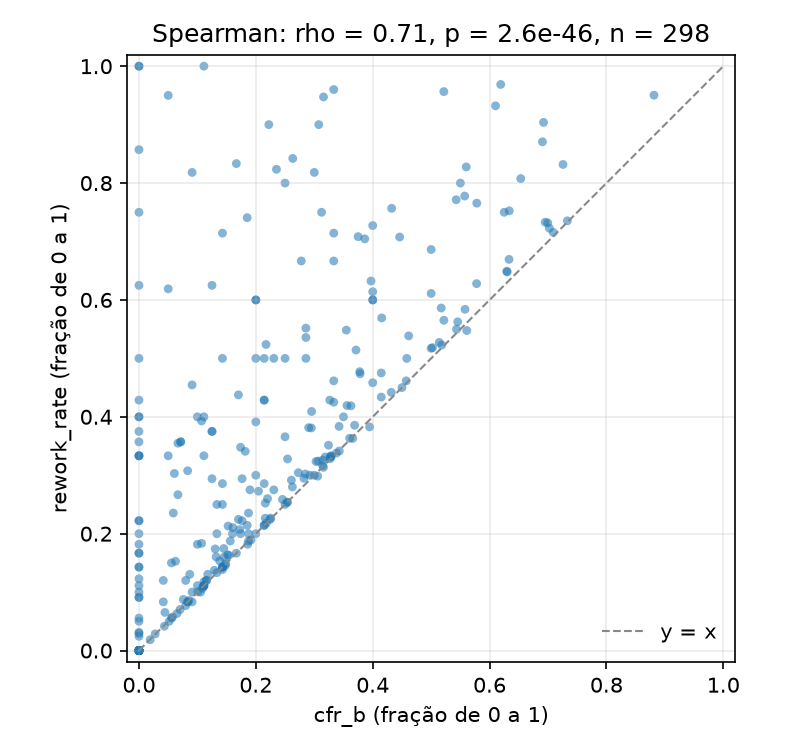
\includegraphics[width=0.55\textwidth]{rq08_cfr_b.png}
\caption{\textit{Rework rate} contra CFR (b) de cada repositório; a linha é a diagonal $y = x$.}
\label{fig:rq08}
\end{figure}

Confirmamos as três hipóteses sobre o \textit{rework rate}: a mediana fica entre 20\% e 40\%, o valor é maior que o do CFR (b) e a correlação com ele é forte. A hipótese sobre a evolução temporal ficou sem teste. O \textit{rework rate} é maior porque conta as releases corretivas publicadas depois dos 7 dias e as que corrigem outra correção, que o CFR (b) não conta, e é a métrica que o DORA adotou em 2024. A correlação forte entre os dois também tem uma causa em comum: ambos dependem da mesma heurística de release corretiva, cujo F1 é de 0,644, e herdam os mesmos erros. Por isso a correlação não prova que os dois medem o mesmo fenômeno, só que erram juntos.


\section{Ameaças à validade}

\paragraph{Construto.} Nenhuma das métricas é observada diretamente. Tratar uma release como deploy só vale se ela chega a quem usa o projeto: o consenso da amostra-ouro foi que sim em 59 dos 60 repositórios, mas com kappa de 0,19 e cobrindo só 60 dos 300 (no \texttt{supabase}, as ``releases'' são boletins mensais). O CFR (a) mede falha de CI, e não de produção; o CFR (b) depende de uma heurística com F1 de 0,644, abaixo da meta de 0,70, com erros nos dois sentidos. O lead time usa a data de autoria do commit, que pode anteceder a sua entrada no ramo (\textit{rebase}, \textit{cherry-pick}), e 6 releases com a tag apagada ou reescrita ficaram fora. A recuperação mede a volta do CI, e não do serviço, e os 0,9\% de episódios censurados não entram na mediana. A RQ 07 dimensiona essa ameaça: a definição muda a categoria de 21,7\% a 30,1\% dos repositórios.

\paragraph{Interna.} A idade tem o maior efeito da RQ 06 (lead time, $\varepsilon^2 = 0{,}365$) e pode se sobrepor a outros fatores, o que a análise por fator isolado não separa. As correlações da RQ 05 não implicam causalidade, e o $\rho$ de 0,501 com o CFR (b) é em parte efeito da definição. As regras da heurística foram escolhidas a partir dos erros nos mesmos 300 itens usados para avaliá-la, o que torna o F1 otimista, e os autores foram também os avaliadores; como mitigação, o protocolo foi escrito antes do sorteio e a rotulagem foi independente e sem ver a saída da heurística.

\paragraph{Externa.} A amostra reúne os 300 repositórios mais populares que passam no funil, e não é um sorteio; as exigências de GitHub Actions, de 5 releases e de 50 execuções favorecem projetos que publicam releases no GitHub. Os resultados não se estendem a projetos pequenos, corporativos ou de outras plataformas, nem necessariamente a outros períodos, e 14 organizações têm mais de um repositório (até 6), o que reduz a independência das observações.

\paragraph{Conclusão.} Só 4 dos 20 testes da RQ 06 permanecem significativos após a correção de Holm, e os do tipo do projeto, com 58 repositórios (o grupo \textit{outro}, com 2, ficou abaixo do mínimo de 5), têm pouco poder. Os quartis são um agrupamento arbitrário, e os testes não paramétricos não ajustam um fator pelos demais. A correlação de Spearman tem muitos empates (11 repositórios com CFR (a) igual a zero e 61 com CFR (b) igual a zero), e o kappa de Fleiss é sensível à prevalência, por isso o de entregas reais é relatado com o acordo bruto (88\%). Por fim, valores próximos de um corte podem mudar de categoria por diferenças pequenas.


\section*{Disponibilidade}

O código, os dados, o dicionário de dados e as análises estão em \url{https://github.com/gabialvarenga/lab-experimentacao-software}, na pasta \texttt{lab03}, e o planejamento das sprints está no quadro do GitHub Projects do mesmo repositório.

\bibliographystyle{sbc}
\bibliography{referencias}

\end{document}
